\section*{Step 6}

\begin{custombox}[label={box:Q6}]{Step 6}
	Compare the metrics within and across the datasets (train and test) and algorithms. In addition to the variations in metrics, include in your report aspects related to classification boundaries, overfitting, etc.
\end{custombox}

\vspace{10mm}

% Dataset 1 is a good separated dataset, 2 is a bit mixed up and 3 is mixed up. 

% \subsection**{Dataset 1}

% In the case of Dataset 1, the training and testing data are well separated. The decision boundaries are clear and the model is not overfitting. The accuracy of the model is $100$\% for both training and testing data for all the $10$ classification models. We also observe that the precision, recall and F1 score are very close to $1.0$ for all the $10$ classification models. Classification boundaries are clear and the model is not overfitting on the training data.

% \subsection**{Dataset 2}

% In the case of Dataset 2, the training and testing data are mixed up. The decision boundaries are not clear and the model is overfitting. The accuracy of the model is $98$\% for the training data and $90$\% on average for the testing data for all the $10$ classification models. We also observe that the precision, recall and F1 score are very close to $1.0$ for all the $10$ classification models. Classification boundaries are not clear and the model is overfitting on the training data.

% \subsection**{Dataset 3}

% In the case of Dataset 3, the training and testing data are  highly mixed up. The decision boundaries are not clear and the model is overfitting. The accuracy of the model is $90$\% for the training data and $90$\% on average for the testing data for all the $10$ classification models. We also observe that the precision, recall and F1 score are very close to $1.0$ for all the $10$ classification models. Classification boundaries are not clear at all and some of the model is overfitting on the training data.

\begin{itemize}
    \item \textbf{Dataset 1:} Clear class separation. We expect simpler models like Logistic Regression and linear SVC to perform well on this dataset.
    \item \textbf{Dataset 2:} Moderate class overlap. Non-linear models such as Random Forest and SVC with rbf kernel are anticipated to outperform linear models.
    \item \textbf{Dataset 3:} Significant class mixing. Complex models like Neural Networks may handle this dataset better due to their ability to capture intricate decision boundaries.
\end{itemize}

\subsection*{Performance Metrics}
We captured the following metrics for each classifier across both the training and test datasets:
\begin{itemize}
    \item \textbf{Accuracy:} Overall accuracy of the model.
    \item \textbf{Precision (per class and average):} The proportion of positive predictions that are actually correct.
    \item \textbf{Recall (per class and average):} The proportion of actual positives that were identified correctly.
    \item \textbf{F1-Score (per class and average):} The harmonic mean of Precision and Recall.
    \item \textbf{AUC (per class and average):} Area Under the Curve, representing the model's ability to distinguish between classes.
\end{itemize}

\subsection*{Results and Discussion}
\subsubsection*{Logistic Regression}
\textbf{Dataset 1:} Logistic Regression performed well due to the clear boundaries between classes, achieving high accuracy and F1-scores for all classes. The linear decision boundary is well-suited for this dataset.

\textbf{Dataset 2:} Performance dropped as class overlap increased, with Precision and Recall averages declining. Logistic Regression struggled to find optimal linear separations between classes.

\textbf{Dataset 3:} The model was unable to effectively classify due to significant overlap, leading to poor AUC and F1-scores. This suggests that the linearity assumption inherent in Logistic Regression is inadequate for this dataset.

\subsubsection*{SVC with Linear Kernel}
\textbf{Dataset 1:} Similar to Logistic Regression, the linear SVC achieved high performance metrics. This confirms the efficacy of linear models for datasets with clear class boundaries.

\textbf{Dataset 2:} The linear kernel began to show limitations, with noticeable drops in precision and recall. The model could not handle the non-linear decision boundaries required for this dataset.

\textbf{Dataset 3:} As expected, performance was poor, with the model showing significant misclassifications due to the inability to capture complex boundaries.

\subsubsection*{SVC with RBF Kernel}
\textbf{Dataset 1:} While SVC with rbf performed slightly better than the linear kernel, the improvement was minimal given that the dataset is linearly separable.

\textbf{Dataset 2:} The rbf kernel significantly improved performance, with higher precision and recall averages compared to the linear SVC. This suggests that non-linear kernels are more effective for datasets with class overlap.

\textbf{Dataset 3:} The model showed substantial improvement over linear methods, capturing non-linear relationships between classes. However, the overall performance still suffered due to the high degree of mixing in the dataset.

\subsubsection*{Random Forest Classifier}
\textbf{Dataset 1:} All variations of the Random Forest Classifier performed exceptionally well, with min\_samples\_leaf=1 achieving the highest accuracy. This is expected due to the ensemble method's robustness to class separation.

\textbf{Dataset 2:} Performance across all Random Forest configurations improved significantly compared to linear models. Increasing min\_samples\_leaf slightly reduced overfitting, especially with min\_samples\_leaf=5, which provided the best test set performance.

\textbf{Dataset 3:} The Random Forest models performed better than linear classifiers but still struggled with the overlapping classes. Increasing the leaf size helped control overfitting to some extent.

\subsubsection*{Neural Networks}
\textbf{Dataset 1:} With a small number of hidden layers, Neural Networks performed comparably to simpler models. However, as the network complexity increased (hidden\_layer\_sizes=(5,5,5)), the model began to overfit the training data.

\textbf{Dataset 2:} The neural networks showed a balanced performance with deeper architectures performing better, especially on the test set. Networks with hidden\_layer\_sizes=(5,5) and (5,5,5) provided the best results.

\textbf{Dataset 3:} The Neural Network with hidden\_layer\_sizes=(10) outperformed all other models, capturing more complex patterns despite the heavy class mixing. However, it still struggled to achieve high precision and recall across all classes due to the inherent data difficulty.

\begin{figure}[H]
    \centering
    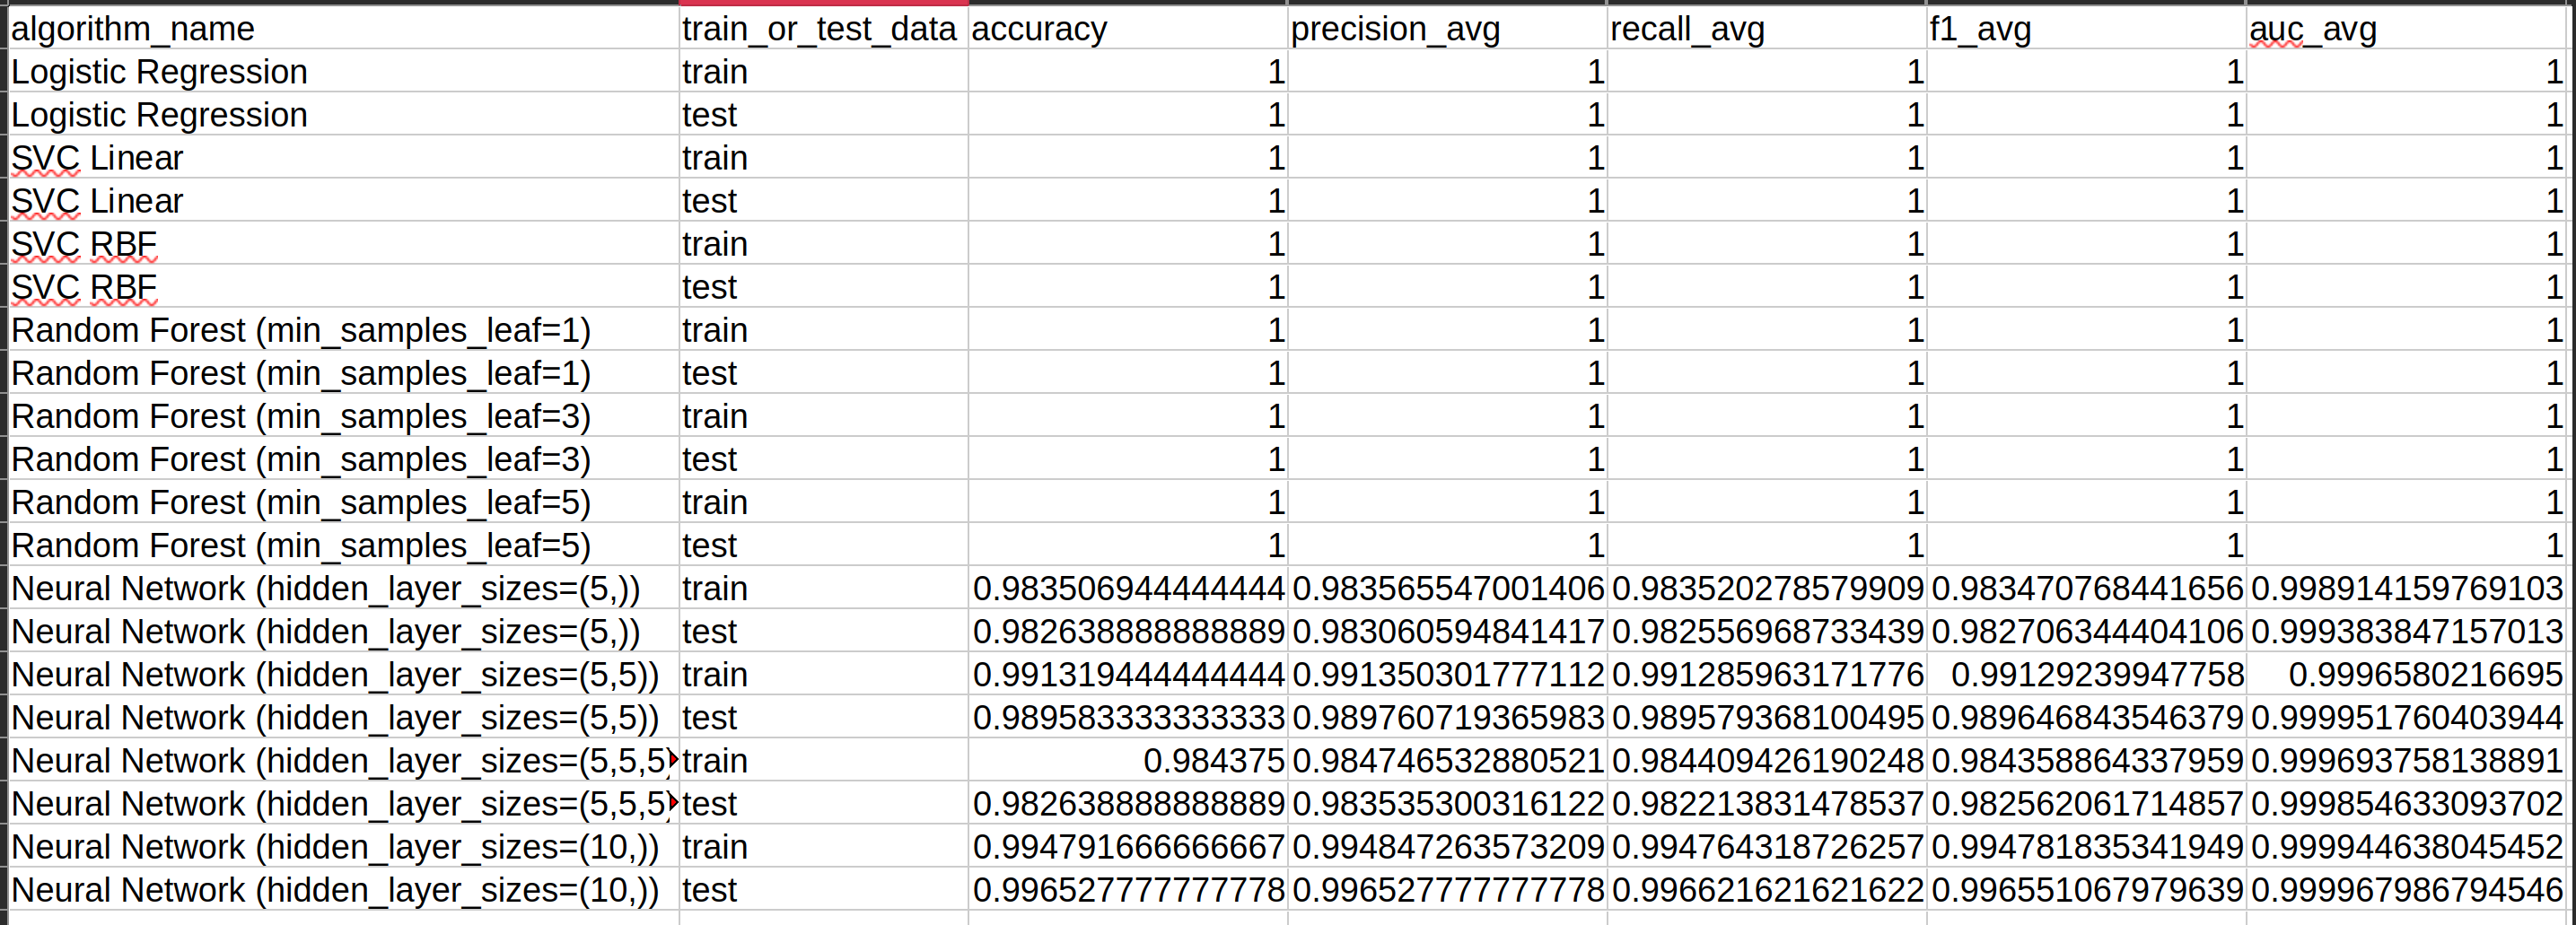
\includegraphics[width=0.8\textwidth]{Images/dataset-1-step6.png}
    \caption{Performance Metrics for Dataset 1}
\end{figure}

\begin{figure}[H]
    \centering
    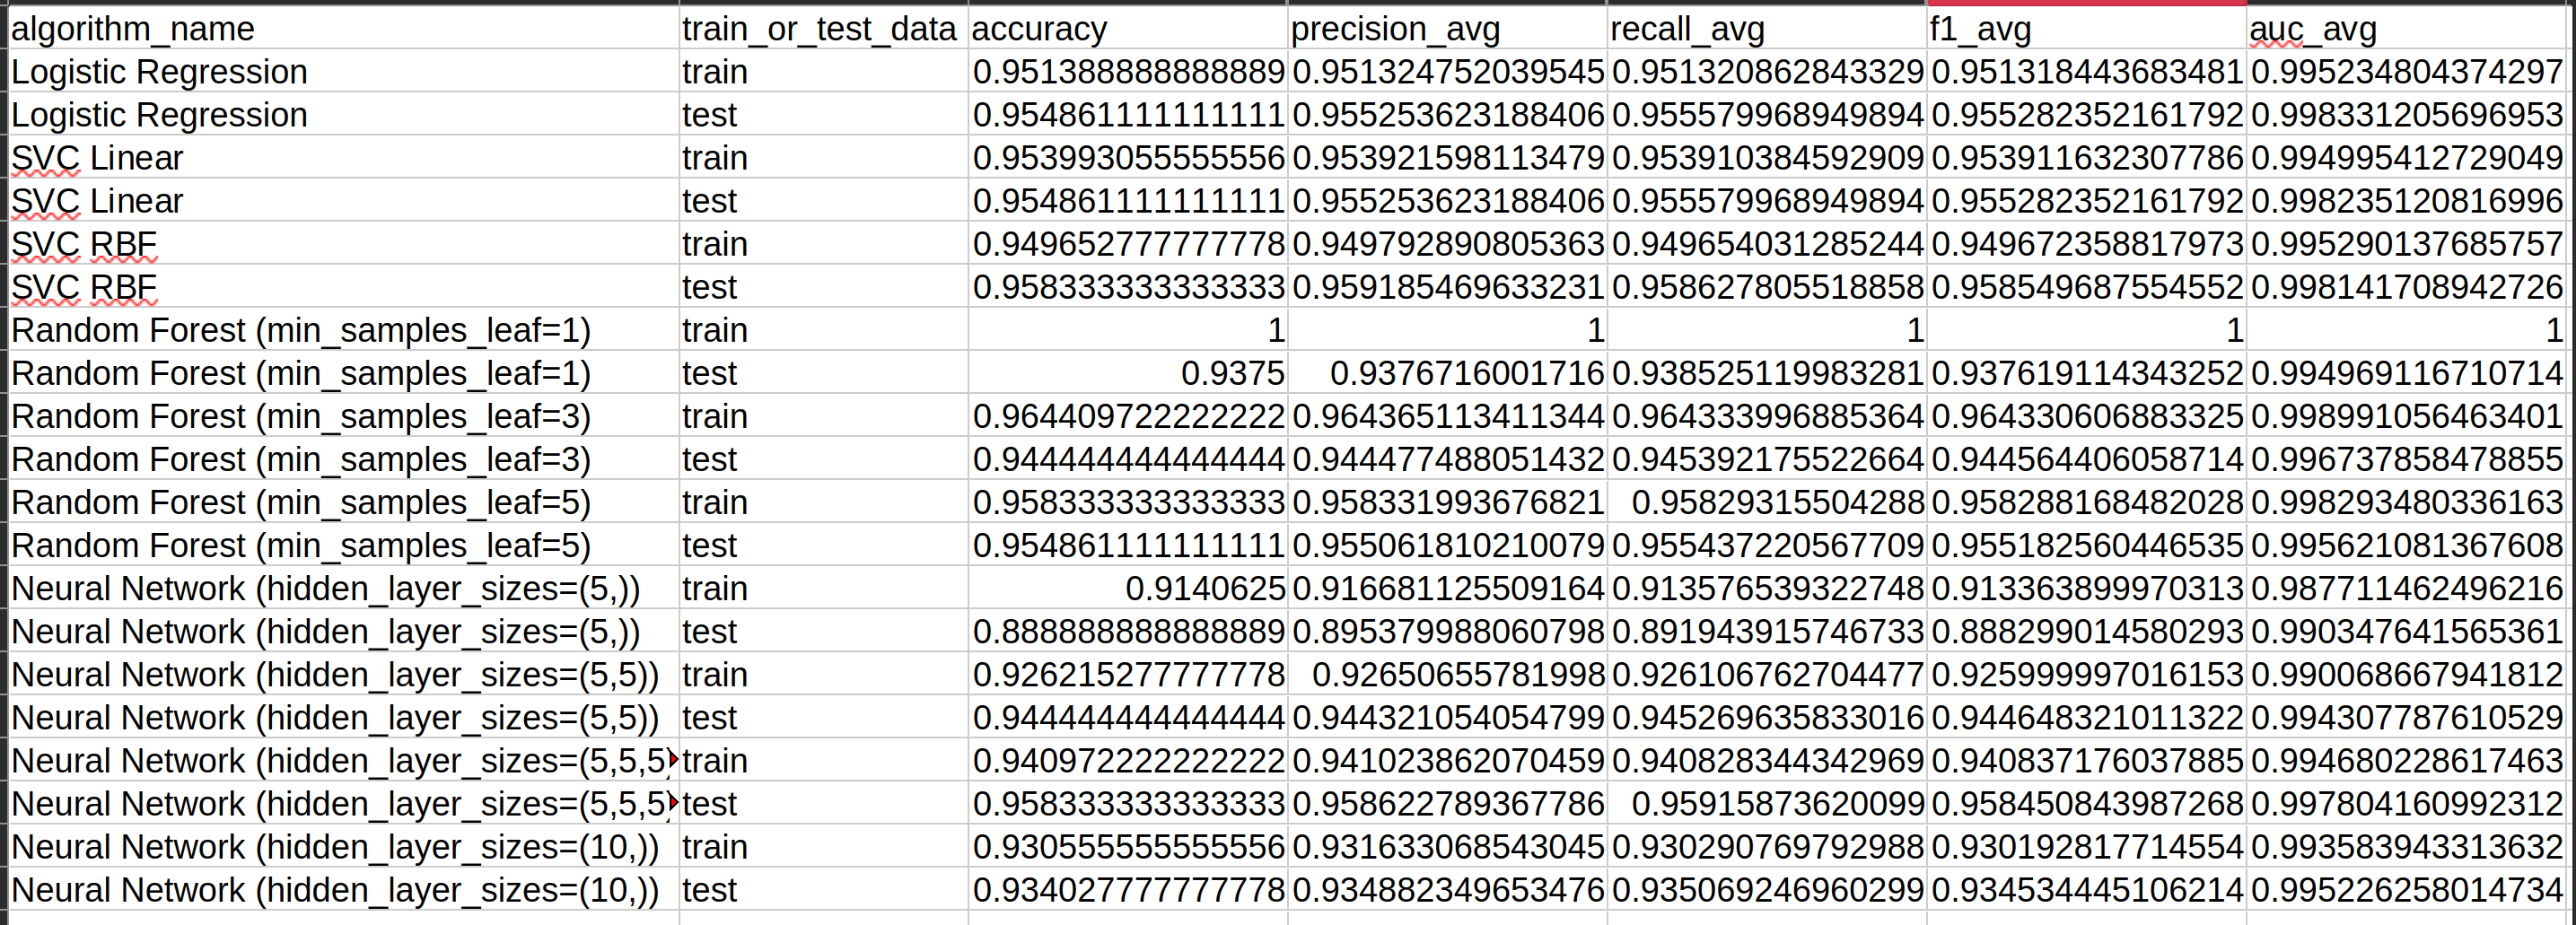
\includegraphics[width=0.8\textwidth]{Images/dataset-2-step6.png}
    \caption{Performance Metrics for Dataset 2}
\end{figure}

\begin{figure}[H]
    \centering
    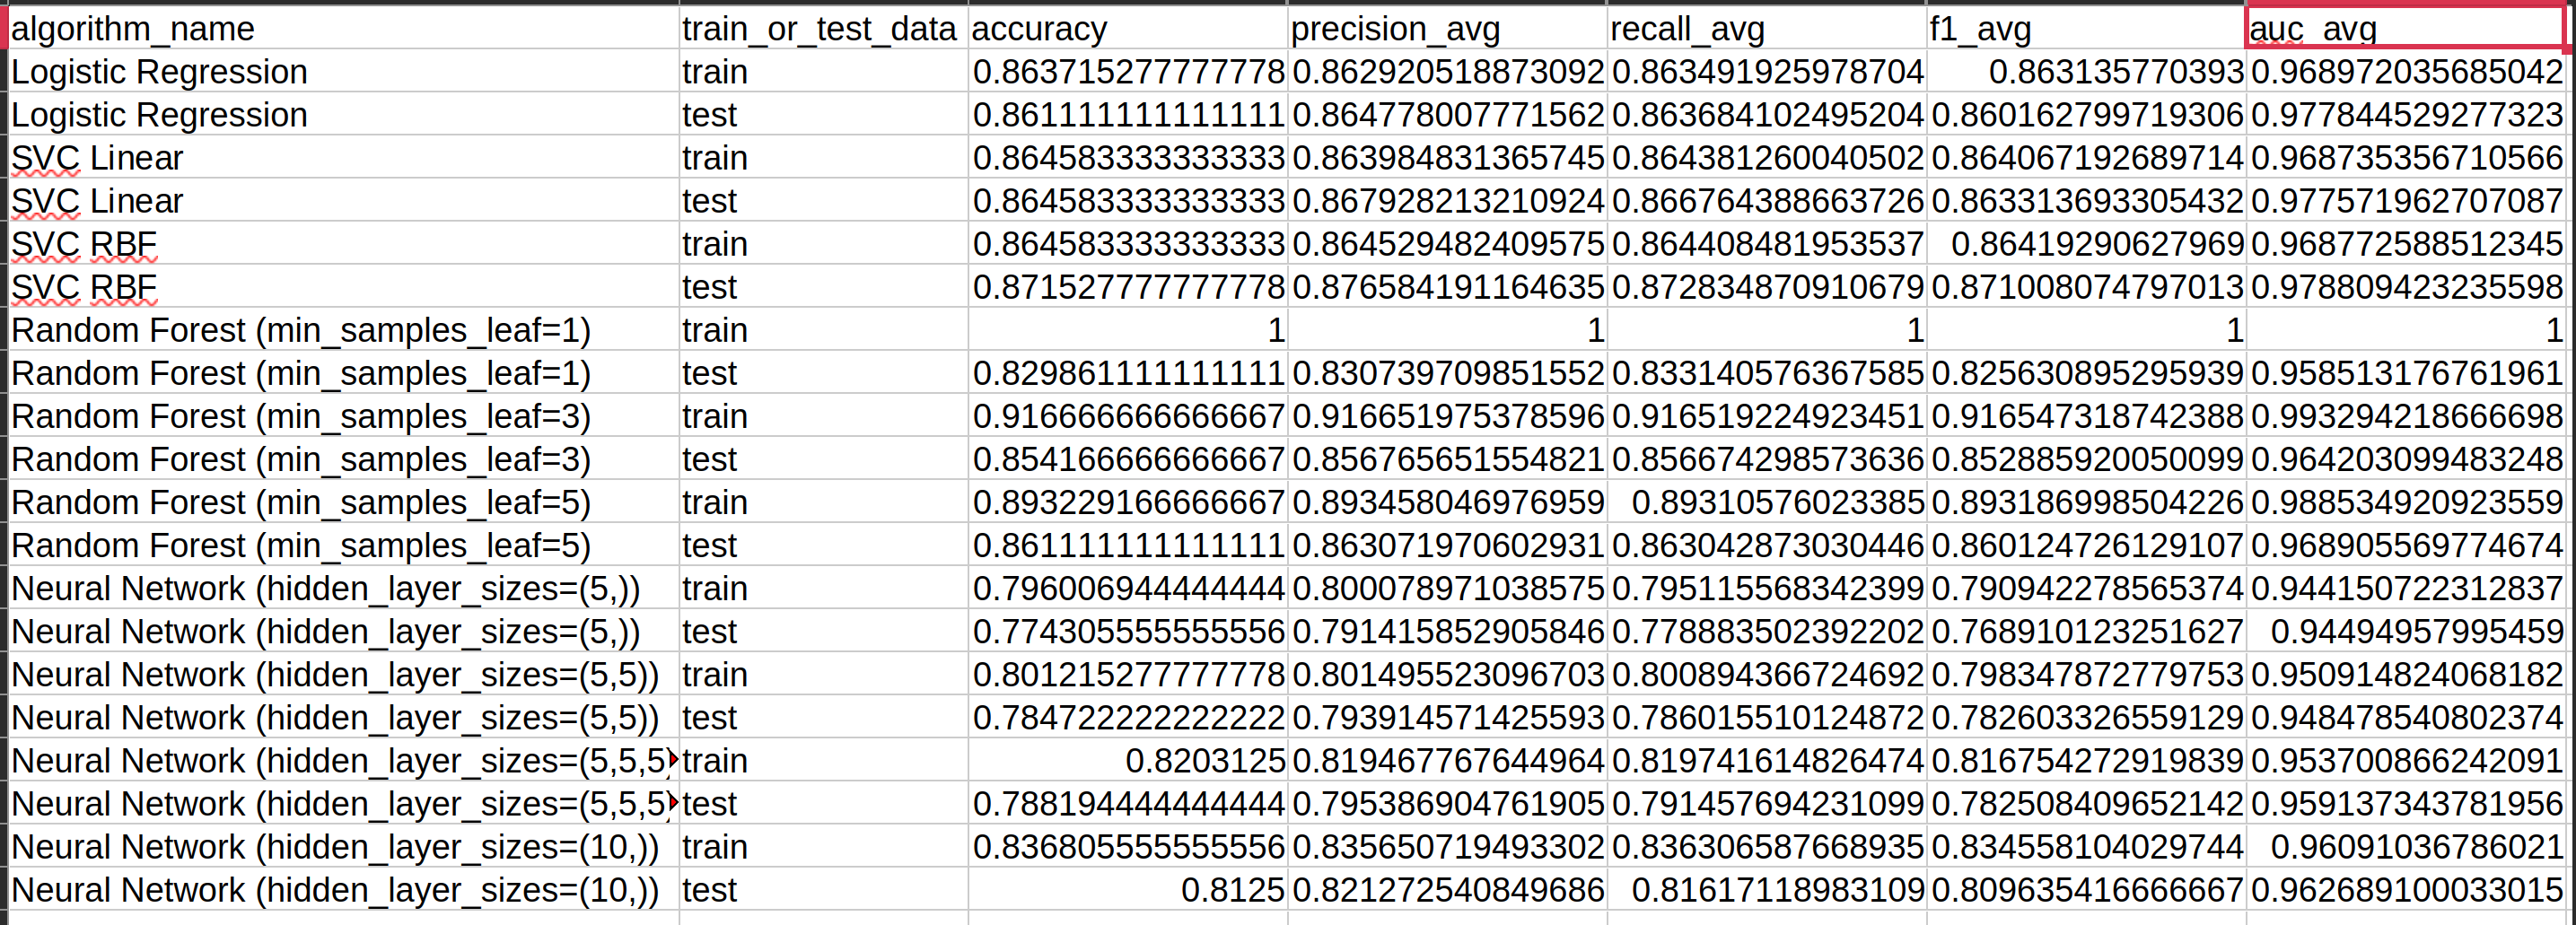
\includegraphics[width=0.8\textwidth]{Images/dataset-3-step6.png}
    \caption{Performance Metrics for Dataset 3}
\end{figure}

\subsection*{Conclusion}
Across all datasets, model performance varied significantly based on the complexity of the data and the classification algorithm used. Logistic Regression and linear SVC excelled on Dataset 1 with clear class separation but failed on more complex datasets. Non-linear models like SVC with rbf kernel and Random Forest performed well on moderately mixed datasets, and Neural Networks showed the best performance on the most complex dataset, albeit with risks of overfitting. Ultimately, model choice should be driven by the nature of the data, with simpler models being more appropriate for clearly separable classes and more complex models like Neural Networks or Random Forests for datasets with significant overlap.




